 \documentclass{eptcs-modified}
\usepackage{amsmath,caption}
\usepackage{tikz,wrapfig}
\usepackage{amssymb}
\usepackage{amsthm}
\usepackage{cleveref,ulem}


\title{Comparing representations for function spaces in computable analysis}
\author{
Arno Pauly
\institute{Computer Laboratory\\ University of Cambridge, United Kingdom \\ \& \\
D\'epartement d'Informatique\\ Universit\'e Libre de Bruxelles, Belgium
\email{Arno.Pauly@cl.cam.ac.uk}}
\and
Florian Steinberg
\institute{Fachbereich Mathematik\\ TU-Darmstadt, Germany
\email{steinberg@mathematik.tu-darmstadt.de}}
}
\def\titlerunning{Comparing representations for function spaces}
\def\authorrunning{A. Pauly \& F. Steinberg}
\newtheorem{theorem}{Theorem}
	\newtheorem{definition}[theorem]{Definition}
	\newtheorem{problem}[theorem]{Problem}
	\newtheorem{assumption}[theorem]{Assumption}
	\newtheorem{corollary}[theorem]{Corollary}
	\newtheorem{proposition}[theorem]{Proposition}
	\newtheorem{lemma}[theorem]{Lemma}
	\newtheorem{observation}[theorem]{Observation}
	\newtheorem{fact}[theorem]{Fact}
	\newtheorem{question}[theorem]{Question}
	\newtheorem{example}[theorem]{Example}
\newcommand{\Wd}[1]{\left[#1\right]}
	\newcommand{\dom}{\operatorname{dom}}
	\newcommand{\adv}{\operatorname{Adv}}
	\newcommand{\Dom}{\operatorname{Dom}}
	\newcommand{\codom}{\operatorname{CDom}}
	\newcommand{\id}{\textnormal{id}}
	\newcommand{\Cantor}{{\{0, 1\}^\mathbb{N}}}
	\newcommand{\Baire}{{\mathbb{N}^\mathbb{N}}}
	\newcommand{\uint}{{[0,1]}}
	\newcommand{\lev}{\textnormal{Lev}}
	\newcommand{\hide}[1]{}
	\newcommand{\mto}{\rightrightarrows}
	\newcommand{\pls}{\textsc{PLS}}
	\newcommand{\ppad}{\textsc{PPAD}}
	\newcommand{\mlr}{\textrm{MLR}}
	\newcommand{\layer}{\textrm{Layer}}
	\newcommand{\blayer}{\textrm{BLayer}}
	\newcommand{\sierp}{Sierpi\'nski}
	\newcommand{\lpo}{\textrm{LPO}}
	\newcommand{\name}[1]{\textsc{#1}}
	\newcommand{\leqW}{\leq_{\textrm{W}}}
	\newcommand{\leqsW}{\leq_{\textrm{sW}}}
	\newcommand{\nleqW}{\nleq_{\textrm{W}}}
	\newcommand{\nleqsW}{\nleq_{\textrm{sW}}}
	\newcommand{\leW}{<_{\textrm{W}}}
	\newcommand{\equivW}{\equiv_{\textrm{W}}}
	\newcommand{\geqW}{\geq_{\textrm{W}}}
	\newcommand{\pipeW}{|_{\textrm{W}}}
	\newcommand{\lay}{\textrm{LAY}}
	\newcommand{\rd}{\textrm{RD}}
	\newcommand{\kol}{\textrm{Kol}}
	\newcommand{\lil}{\textrm{LIL}}
	\newcommand{\CCN}{\mathrm{C}_{\NN}}
	\newcommand{\demph}{\textbf}
	\newcommand{\C}{\textrm{C}}
	\newcommand{\NN}{\mathbb{N}}
	\newcommand{\sir}{\mathbb{S}}
	\newcommand{\RR}{\mathbb{R}}
	\newcommand{\KK}{\mathbb{K}}
	\newcommand{\CC}{\mathbb{C}}
	\newcommand{\DD}{\mathbb{D}}
	\newcommand{\HH}{\mathcal{H}}
	\newcommand{\OO}{\mathcal{O}}
	\newcommand{\XX}{\mathbf{X}}
	\newcommand{\YY}{\mathbf{Y}}
	\newcommand{\EE}{\mathcal E}
	\newcommand{\SF}{\mathcal S}
	\newcommand{\TF}{\mathcal D}
	\newcommand{\A}{\mathcal A}
	\newcommand{\abs}[1]{\left|#1\right|}
	\newcommand{\germs}{\OO}
	\newcommand{\Sum}{\operatorname{Sum}}
	\newcommand{\analytic}{\mathcal C^\omega(D)}
	\newcommand{\cont}{\mathcal C(D)}
	\newcommand{\Advc}{\operatorname{Adv}_{\C^\omega}}
	\newcommand{\Advg}{\operatorname{Adv}_{\germs}}
	\newcommand{\Count}{\operatorname{Count}}
	\newcommand{\Bound}{\operatorname{Bound}}
	\newcommand{\Germ}{\operatorname{Germ}}
	\newcommand{\Diff}{\operatorname{Diff}}
	\newcommand{\supp}{\operatorname{supp}}
	\newcommand{\Monic}{\operatorname{Monic}}
	\newcommand{\Zeros}{\operatorname{Zeros}}
	\newcommand{\Zeroapprox}{\operatorname{Zeroapprox}}
	\newcommand{\dbnd}{\operatorname{Dbnd}}
	\newcommand{\card}[1]{\#{#1}}
	\newcommand{\norm}[1]{\left\|#1\right\|}
	\newcommand{\bnorm}[1]{\big\|#1\big\|}

\begin{document} \theoremstyle{definition}

	\maketitle

	\begin{abstract}
		This paper compares different representations (in the sense of computable analysis) of a number of function spaces that are of interest in analysis.
		In particular subspace representations inherited from a larger function space are compared to more natural representations for these spaces.
		The formal framework for the comparisons is provided by Weihrauch reducibility.

		The centrepiece of the paper considers several representations of the analytic functions on the unit disk and their mutual translations.
		All translations that are not already computable are shown to be Weihrauch equivalent to closed choice on the natural numbers.
		Subsequently some similar considerations are carried out for representations of polynomials.
		In this case in addition to closed choice the Weihrauch degree  shows up as the difficulty of finding the degree or the zeros.
		As a final example, the smooth functions are contrasted with functions with bounded support and Schwartz functions.
		Here closed choice on the natural numbers and the  degree appear.
\end{abstract}
	\tableofcontents

	\section{Introduction}
		In order to make sense of computability questions in analysis, the spaces of objects involved have to be equipped with representations:
		A representation determines the information that is provided (or has to be provided) when computing on these objects.
		When changing from a more general to more restrictive setting, there are two options:
		Either to merely restrict the scope to the special objects and retain the representation, or to introduce a new representation containing more information.

		As a first example of this, consider the closed subsets of  and the closed convex subsets of  (following \cite{paulyleroux}).
		The former are represented as enumerations of open balls exhausting the complement.
		The latter are represented as the intersection of a decreasing sequence of rational polygons.
		Thus, prima facie the notions of a \emph{closed set which happens to be convex} and a \emph{convex closed set} are different.
		In this case it turns out they are computably equivalent after all (the proof, however, uses the compactness of ).

	\subsection{Summary of the results}
		This paper presents different examples of the same phenomenon:
		In \Cref{sec:analytic} the difference between an \emph{analytic function} and a \emph{continuous functions that happens to be analytic} is investigated for functions on a fixed compact domain.
		It is known that these actually are different notions.
		The results quantify how different they are using the framework of Weihrauch reducibility.
		The additional information provided for an analytic function over a continuous function can be expressed by a single natural number.
		Thus, this is an instance of computation with discrete advice as introduced in \cite{MR2915702}.
		Finding this number is Weihrauch equivalent to .
		This means that while the number can be chosen to be falsifiable (i.e.~wrong values can be detected), this is the only computationally relevant restriction on how complicated the relationship between object and associated number can be.
		The results are summarized in \Cref{figure:reductions} on Page \pageref{figure:reductions}

		\Cref{sec:polynomials} considers \emph{continuous functions that happen to be polynomials} versus \emph{analytic functions that happen to be polynomials} versus \emph{polynomials}.
		All translations turn out to be either computable, or Weihrauch equivalent to one of the two well-studied principles  and .
		The results are summarized in \Cref{figure:reductions for polynomials} on Page \pageref{figure:reductions for polynomials}.

		The last \Cref{sec:schwartz} changes the setting in that it swaps the compact subset of the complex plane as domain for the real line.
		It contrasts the spaces of smooth functions, Schwartz functions and bump functions.
		While going from smooth (or Schwartz) to a bump function is equivalent to , going from a smooth function that happens to be Schwartz to a Schwartz function is equivalent to the Weihrauch degree .
		This degree captures the Halting problem.
		In particular it follows that there is a function  that decays faster than any polynomial (i.e. ) and is computable as element of , but as element of  is not only  non-computable, but computes the Halting problem.

		We briefly mention two alternative perspectives on the phenomenon:
		First, recall that in intuitionistic logic a negative translated statement behaves like a classical one, and that double negations generally do not cancel.
		In this setting the difference boils down to considering either analytic functions or continuous functions that are not not analytic.
		Second, from a topological perspective, Weihrauch equivalence of a translation to  implies that the topologies induced by the representations differ.
		Indeed, the suitable topology on the space of analytic functions is not just the subspace topology inherited from the space of continuous functions but a direct limit topology.

		An extended abstract based on this paper can be found as \cite{pauly-steinberg-csr}.

		\subsection{Represented spaces}
			This section provides a very brief introduction to the required concepts from computable analysis.
			For a more in depth introduction and further information, the reader is pointed to the standard textbook in computable analysis \cite{MR1795407}, and to \cite{pauly-synthetic}.
			Also, \cite{MR1005942} should be mentioned as an excellent source, even though the approach differs considerably from the one taken here.
		
			Recall that a \demph{represented space}  is given by a set  and a partial surjection  from Baire space onto it.
			The elements of  should be understood as encodings of  and are called the \demph{-names} of .
			Each represented spaces inherits a topology from Baire space:
			The final topology of the chosen representation.
			We usually refrain from mentioning the representation of a represented space in the same way as the topology of a topological space is usually not mentioned.
			For instance the set of natural numbers is regarded as a represented space with the representation .
			Therefore, from now on denote by  not only the set or the topological space, but the \demph{represented space of natural numbers}.
			If a topological space is to represented, the representation should be chosen such that it fits the topology as good as possible.
			For instance for the case  above, the final topology of the representation is the discrete topology.

			If  is a represented space and  is a subset of , then  can be turned into a represented space by equipping it with the range restriction of the representation of .
			Denote the represented space arising in this way by .
			We use the same notation  if  is a represented space already.
			In this case, however, no information about the representation of  is carried over to .
			
			Recall that a multivalued function  from  to  (or  to ) is an assignment that assigns to each element  of its domain a set  of acceptable return values.
			Multivaluedness of a function is indicated by .
			The domain of a multivalued function is the set of elements such that the image is not empty.
			Furthermore, recall that  indicates that the function  is allowed to be partial, i.e. that its domain may be a proper subset of .

			\begin{definition}
				A partial function  is a \demph{realizer} of a multivalued function  if  for all  (compare \Cref{figure:diagram}).
			\end{definition}
			
			\begin{wrapfigure}{r}{3.4cm}
				\vspace{-.5cm}
				\begin{tikzpicture}
					\node at (0,0) {};
					\node at (0,1.5) {};
					\node at (2,0) {};
					\node at (2,1.5) {};
					\draw[->] (0.3,1.5) -- (1.7,1.5);				
					\draw[->] (0,0.3) -- (0,1.2);
					\draw[->] (2,0.3) -- (2,1.2);
					\draw[->] (0.3,0) -- (1.55,0);
					\node at (1,1.8) {};
					\node at (-.3,.75) {};
					\node at (2.3,.75) {};
					\node at (1,-.3) {};
				\end{tikzpicture}
				\caption{A diagram}\label{figure:diagram}
				\vspace{-.8cm}
			\end{wrapfigure}
			A (multivalued) function between represented spaces is called computable if it has a computable realizer, where computability on Baire space is defined via oracle Turing machines (as in e.g.~\cite{MR1673610}) or via Type-2 Turing machines (as in e.g.~\cite{MR1795407}).
			We call a (multivalued) function between represented spaces continuous, if it has a continuous realizer.
			For single valued functions on admissibly represented spaces (in the sense of Schr\"oder \cite{schroder}), this notion coincides with topological continuity.
			All representations discussed in this paper are admissible.		

			The remainder of this section introduces the represented spaces that are needed for the content of the paper.

			\subsubsection*{Sets of natural numbers.}

				Let  resp.\  denote the \demph{represented spaces of open} resp.\ \demph{closed subsets of }.
				The underlying set of both  and  is the power set of .
				The representation of  is defined by
				
				That is: A -name of a set of natural numbers is an enumeration of the set, however the enumeration is allowed to not return an element of the set in each step (otherwise no finite set would get a name).
				The closed sets  are represented as complements of open sets:
				
				I.e. a -name of a set of natural numbers is an enumeration of the complement.
		


			\subsubsection*{Computable metric spaces, , , .}
				Given a triple  such that  is a separable metric space and  is a dense sequence, turn  into a represented space by equipping it with the representation
				
				This is the canonical way of considering ,  and  as represented spaces; the dense sequences are standard enumerations of the rational elements.

				The space  of continuous functions on a compact subset  of  is a separable metric space and thus a represented space.
				The metric is the one induced by the supremum norm and the dense sequences are standard enumerations of the polynomials with rational coefficients.
				The computable Weierstra\ss\ approximation theorem states that a function is computable as element of  if and only if it is computable in the sense of realizers as a function between the represented spaces  and  respectively.

			\subsubsection*{Sequences in a represented space.}

				For a represented space  there is a canonical way to turn the set of sequences in  into a \demph{represented space }:
				Let  be a standard paring function (i.e. bijective, recursive with recursive projections).
				Define a function  by
				
				For a represented space  define a representation of the set  of the sequences in the set  underlying  by
				
				I.e.  is a name of  if for each fixed  the mapping  is a name of .
				In particular the spaces  and  of real and complex sequences are considered represented spaces in this way.
				For a partial, multivalued function  let  denote the function defined by .

		\subsection{Weihrauch reducibility}
			This section provides a brief introduction to Weihrauch reducibility.
			The research programme of Weihrauch reducibility was formulated in \cite{MR2099383}, a more up-to-date introduction can be found in \cite{MR3350999}.

			Every multivalued function  corresponds to a computational task.
			Namely: \lq given information about  and the additional assumption  find suitable information about some \rq.
			What information about  resp.\  is provided resp.\ asked for is reflected in the choice of the representations for  and .
			The following example of this is very relevant for the content of this paper:
			\begin{definition}
				Let \demph{closed choice on the integers} be the multivalued function  defined on nonempty sets by
				
			\end{definition}
			The corresponding task is \lq given an enumeration of the complement of a set of natural numbers and provided that it is not empty, return an element of the set\rq.
			 does not permit a computable realizer:
			Whenever a machine decides that the name of the element of the set should begin with , it has only read a finite beginning segment of the enumeration.
			The next value might as well be .

			From the point of view of multivalued functions as computational tasks, it makes sense to compare their difficulty by comparing the corresponding multivalued functions.
			This paper uses Weihrauch reductions as formalization of such a comparison.
			Weihrauch reductions define a rather fine pre-order on multivalued functions between represented spaces.

			\begin{wrapfigure}{r}{3.5cm}
				\vspace{-.2cm}
				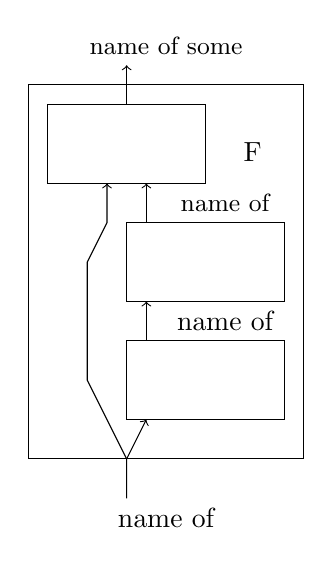
\begin{tikzpicture}
					\node at (.5,4.75) {\small{name of some }};
					\draw (-1.25,-.5) rectangle (2.25,4.25);
					\draw (0,0) rectangle (2,1);
					\node at (1,.5) {};
					\draw[->] (0,-.5) -- (.25,0);
					\node at (.5,-1.25) {name of };
					\draw[->] (.25,1) -- (.25,1.5);
					\node at (1.25,1.25) {name of };
					\draw (0,1.5) rectangle (2,2.5);
					\node at (1,2) {};
					\node at (1.25,2.75) {\small{name of }};
					\draw[->] (.25,2.5) -- (.25,3);
					\draw[->] (0,-1) -- (0,-.5) -- (-.5,.5) -- (-.5,2) --(-.25,2.5) --(-.25,3);
					\draw (-1,3) rectangle (1,4);
					\node at (0,3.5) {};
					\draw[->] (0,4) -- (0,4.5);
					\node at (1.6,3.4) {F};
				\end{tikzpicture}
				\caption{Weihrauch reductions}\label{fig:Wheirauch reduction}
				\vspace{-.8cm}
			\end{wrapfigure}
			
			\begin{definition}\label{def:weihrauch}
				Let  and  be partial, multivalued functions between represented spaces.
				Say that  is \demph{Weihrauch reducible} to , in symbols , if there are computable
				functions  and  such that whenever  is a realizer of , the function  is a realizer for .
			\end{definition}

			 is called the \demph{pre-processor} and  the \demph{post-processor} of the Weihrauch reduction.
			This definition and the nomenclature is illustrated in \Cref{fig:Wheirauch reduction}.
			The relation  is reflexive and transitive.
			We use  to denote that reductions in both directions exist and  if this is not the case.
			The equivalence class of a multivalued function with respect to the equivalence relation  is called the \demph{Weihrauch degree} of a function  and we denote it by .
			We still use  for the induced partial order on the Weihrauch degrees and by abuse of notations sometimes use it to compare multivalued functions and Weihrauch degrees.
			A Weihrauch degree is called non-computable if it contains no computable function.

			The Weihrauch degree corresponding to  has received significant attention, e.g.~in \cite{MR2760117,MR2915694,paulymaster,mylatz,mylatzb,MR3350999,paulyoracletypetwo,mummert,paulyneumann}.
			In particular, as shown in \cite{paulydebrecht}, a function between computable Polish spaces is Weihrauch reducible to  if and only if it is piecewise computable or equivalently is effectively -measurable.
			
			For the purposes of this paper, the following representatives of this degree are also relevant:
			\begin{lemma}[\cite{pauly-fouche2}]\label{lemma:cn}
				The following are Weihrauch equivalent:
				\begin{itemize}
					\item , that is closed choice on the natural numbers.
					\item  defined on the bounded sets in the obvious way.
					\item , where  iff .
				\end{itemize}
			\end{lemma}

			Given  denote the support of  by .
			Furthermore, for a finite set  denote the number of elements of that set by .
			\begin{lemma}\label{lemma:count}
				The function , defined via
				
				is Weihrauch equivalent to closed choice on the naturals .
			\end{lemma}

			\begin{proof}
				First construct the Weihrauch reduction that proves :
				Let the pre-processor  be the function sending some  to the function that returns  on input  whenever its support up to  has fewer elements than the least element that has not been excluded from the set by the first  elements of the enumeration of the complement.
				This function is computable as can be seen from its recursive definition:
				
				 has finite support, since the set described by  is nonempty:
				There is some  never shows up as value of  and by definition the support of  does not outgrow that number.
				Applying a realizer of  to  returns an encoding of the least element of the set encoded by .
				To obtain a Weihrauch reduction just pass this number on to be the output via .
				
				For the opposite direction, i.e.  use \Cref{lemma:cn} and replace  by .
				Define the pre-processor  of a Weihrauch reduction  as follows:
				
				This means that  is a  name of .
				Applying  will give the maximal element of the support.

				Define the post-processor  to be the function
				
				This function is computable and since  will always be the maximal element of the support of , the composition counts the support of  and is a Weihrauch reduction.
			\end{proof}

			In Section \ref{sec:polynomials} another non-computable Weihrauch degree is encountered: .
			Here,  is short for \lq limited principle of omniscience\rq.
			We refrain from stating  explicitly as it would need more machinery than we introduced.
			Instead we characterize it by specifying the representative that is used in the proofs:
			\begin{proposition}[{\cite[Korollar 3.1.4.6]{paulymaster}}]\label{resu:lpo*}
				The function  defined on all of Baire space in the obvious way is a representative of the Weihrauch degree .
			\end{proposition}

			A third and final Weihrauch degree making an appearance as the degree of a translation is the degree  encountered in Section \ref{sec:schwartz}.

			\begin{definition}
				Let  be a computable metric space.
				Then  maps a converging sequence to its limit.
			\end{definition}

			As shown in \cite{MR2915694}, .
			In general, it holds that , and whenever  is a subspace of , then .
			As  embeds into any computable metric space considered in this paper apart from , it suffices to consider the Weihrauch degree  corresponding to .
			The degree  is also complete for the effectively -measurable functions \cite{MR2099383,pauly-descriptive}.

			To give more intuition as to why the Weihrauch degrees ,  and  show up in this paper, note the following:
			All three are derived from the maybe simplest non-computable Weihrauch degree  via canonical closure operators defined on the Weihrauch degrees.
			 the Weihrauch degree of the characteristic function of the zero function in Baire space, namely , where
			
			In computable analysis  shows up as the Weihrauch degree of the equality test for real (or complex) numbers.

			Now,  corresponds to carrying out a fixed finite but arbitrary high number of equality tests on the real or complex numbers via the operator  from \cite{paulyreducibilitylattice}.
			The operator  introduced in \cite{paulyneumann} captures using the given degree an arbitrary finite number of times (without the requirement that the number is fixed in advance), and it holds that .
			Define one last operator on the Weihrauch degrees by setting .
			This operation was also investigated in \cite{brattka2} and corresponds to a countable number of invocations of  all performed in parallel.
			It holds that .

			It is known that .

	\section{Analytic functions}\label{sec:analytic}
		\subsection{Representations of analytic functions}\label{sec:analytic functions}

			Recall that a function is analytic if it is locally given by a power series:
			\begin{definition}
				Let  be a set.
				A function  is called \demph{analytic}, if for every  there is a neighborhood  of  and a sequence  such that for each 
				
			\end{definition}
			The set of analytic functions is denoted by .
			Each analytic function is continuous, i.e. .
			If  is open, the analytic functions on  are smooth, i.e. infinitely often differentiable.
			Any analytic function can be analytically extended to an open superset of its domain.

			Recall that a \demph{germ} of an analytic function is a point of its domain together with the series expansion around said point.
			As long as the domain is connected, an analytic function is uniquely determined by each of its germs.
			The one to one correspondence of germs and analytic functions only partially carries over to the computability realm:
			It is well known that an analytic function on the unit disk is computable if and only if the germ around any computable point of the domain is computable (see for instance \cite{MR1137517}).
			However, the proofs of these statements are inherently non-uniform.
			The operations of obtaining a germ from a function and a function from a germ are discontinuous and therefore not computable (see \cite{Muller1995}).

			There is a more suitable representation for the analytic functions than the restriction of the representation of continuous functions.
			This representation has been investigated by different authors for instance in \cite{MR3377508},\cite{MR2207129},\cite{Muller1995}.
			For simplicity restrict to the case of analytic functions on the unit disk.
			From now on let  denote the closed unit disk.
			And let  denote the open ball   of radius  around zero.
			Note that  and that the intersection of all  is the unit disk.
			Recall from the introduction that the space  of continuous functions is represented as a metric space (where  is identified with ).
			\begin{definition}\label{def:analytic rep}
				Let  denote the \demph{represented space of analytic functions on }, where the representation is defined as follows:
				A function  is a name of an analytic function  on , if and only if  extends analytically to the closure of , the extension is bounded by  and  is a name of .
			\end{definition}

			Note that the representation of  arises from the restriction of the representation of continuous functions by adding discrete additional information.
			This information is quantified by the advice function  whose domain are the analytic functions and that on those is defined by
			
			This function turns up in the results of this paper.
			In the terminology of \cite{MR3377508}, one would say that  arises from the restriction  by enriching with the discrete advice .

			The topology induced by the representation of  is well known and used in analysis:
			It can be constructed as a direct limit topology and makes  a so called Silva-Space.
			For more information on this topology and its relation to computability and complexity theory also compare \cite{MR2207129}.

			The set  of germs around zero, i.e. of power series with radius of convergence strictly larger than  can be made a represented space in a very similar way:
			\begin{definition}
				Let  denote the represented space of germs around zero with radii of convergence greater than , where the representation is defined as follows: A function  is a name of a power series , if and only if
				
				and  is a name of the sequence  as element of .
			\end{definition}

			As above, this representation is related to the restriction of the representation of  by means of an advice function  whose domain are the sequences with radius of convergence strictly larger than one and that is defined on those by
			
			Again, the topology induced by this representation is well known and used in analysis: It is the standard choice of a topology on the set of germs and can be introduced as a direct limit topology.

			Proofs that the following holds can be found in \cite{MR3377508} or \cite{Muller1995}:
			\begin{theorem}[computability of summation]\label{thm:analytic rep}
				The assignment
				
				is computable.
			\end{theorem}
			A proof of the following can be found in \cite{MR3377508}:
			\begin{theorem}\label{thm:differntiation}
				Differentiation is computable as mapping from  to .
			\end{theorem}

		\subsection{Summing power series}\label{sec:sub:summing power series}
			Summing a power series is not computable on .
			Recall that  was the advice function of the representation  of germs around zero of analytic functions on the unit disk.
			The computational task corresponding to this multivalued function is to find from a sequence that is guaranteed to have radius of convergence bigger than one a constant witnessing the exponential decay of the absolute value of the coefficients (compare \cref{eq:AG} on page \pageref{eq:AG}).
			\Cref{thm:analytic rep} states that summation is computable on .
			Therefore, the advice function  can not be computable.
			The following theorem classifies the difficulty of summing power series and  in the sense of Weihrauch reductions.

			\begin{theorem}\label{thm:main germs}
				The following are Weihrauch-equivalent:
				\begin{itemize}
					\item \textbf{}, that is: Closed choice on the naturals.
					\item \textbf{}, that is: The partial mapping from  to  defined on the sequences with radius of convergence strictly larger than one by
					
					I.e. summing a power series.
					\item \textbf{}, that is: The function from \cref{eq:AG} on page \pageref{eq:AG}. I.e. obtaining the constant from the series.
				\end{itemize}
			\end{theorem}

			\begin{proof}
			Build a Weihrauch reduction circle:
				\begin{description}
					\item[:]
					\Cref{lemma:count} permits to replace  by .

					The Weihrauch reduction  can be constructed as follows:
					Let the pre-processor be a realizer of the computable mapping that assigns to  the sequence  defined by
					
					Note that  means that  has a finite support, and the radius of convergence of  is strictly bigger than one (it is infinite).
					Applying a realizer of  will result in a name of the corresponding function .
					From the definition of  it is clear that .
					Therefore, the post-processor can be chosen as the second projection composed with a realizer of the evaluation in , which is well known to be computable on the continuous functions.
				\item[:]
					Let the pre-processor be the identity.
					Note that an element of  and a -name of  can easily be put together to an -name of .
					Thus the post-processor can be chosen to be the composition of this mapping and a realizer of the summation mapping on , which is computable by \Cref{thm:analytic rep}.
				\item[:]
					Let the pre-processor be the function that maps a given name  of  to an -name of the set .
					Note that an enumeration of the complement of this set can be extracted from  as follows:
					For all  and  dovetail the test .
					If it holds for some , return  as an element of the complement.
					This procedure indeed produces a list of the complement of :
					If the above does not hold for any , then  for all  and  is an element of .

					Applying closed choice to this set will give result in a valid return value.
					Thus, choose the post-processor to be the second projection.
				\end{description}
			\end{proof}

		\subsection{Differentiating analytic functions}

			In \Cref{sec:analytic functions} we remarked that it is not possible to compute the germ of an analytic function just from a name as continuous function.
			The proof in \cite{Muller1995} that this is in general impossible, however, argues about analytic functions on an interval.
			The first lemma of this chapter proves that for analytic functions on the unit disk it is possible to compute a germ if its base point is well inside of the domain.
			We only consider the case where the base point is zero, but the proof works whenever a lower bound on the distance of the base point to the boundary of the disk is known.

			\begin{lemma}\label{lemma:computing germ}
				, that is: The partial mapping from  to  defined on analytic functions by mapping them to their series expansion around zero, is computable.
			\end{lemma}

			\begin{proof}
				Remember that the Cauchy integral formula states that for an analytic function  on the closed unit disk:
				
				It is well known that the integral is computable from a name of the function .
				This works uniformly in .
			\end{proof}

			The next theorem is very similar to \Cref{thm:main germs}.
			Both the advice function  and computing a germ around a boundary point are shown to be Weihrauch equivalent to .
			Note that the coefficients of the series expansion  of an analytic function  around a point  are related to the derivatives  of the function via .
			Therefore, computing a series expansion around a point is equivalent to computing all the derivatives in that point.

			\begin{theorem}\label{thm:main functions}
				The following are Weihrauch equivalent:
				\begin{itemize}
					\item \textbf{}, that is closed choice on the naturals.
					\item \textbf{}, that is the partial mapping from  to  defined on analytic functions by
					
					I.e. evaluating the derivative of an analytic function in .
					\item \textbf{}, that is the function from \cref{eq:AC}. I.e. obtaining the constant from the function.
				\end{itemize}
			\end{theorem}

			\begin{proof}
				By building a circle of Weihrauch reductions:
				\begin{description}
					\item[:]
						Use \Cref{lemma:count} and show  instead.
						Let  be an element of the do- \quad

						\noindent\begin{minipage}{.6\textwidth}
main of .
							That is:  is finite.
							Define a sequence of analytic functions  by
							
							where
							
							(see \Cref{fig:the functions fn}). The sequence is carefully chosen such that
						\end{minipage}\hspace{.25cm}
						\begin{minipage}{.3\textwidth}
							\vspace{-.1cm}
							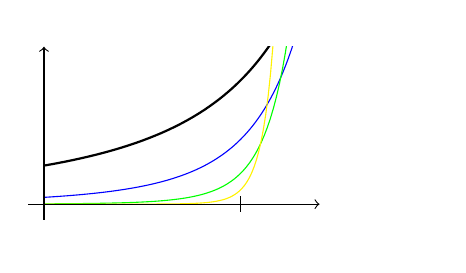
\begin{tikzpicture}
								\begin{scope}
									\clip (0,0) rectangle (5,2);
									\draw[color=black,thick] plot[samples=100,domain=0:1.5] ({2.5*\x},{(\x-1-2^(1/3))^(-2)*2.5});
									\draw[color=blue,] plot[samples=100,domain=0:1.5] ({2.5*\x},{(\x-1-2^(2/5))^(-4)*2.5});
									\draw[color=green] plot[samples=100,domain=0:1.5] ({2.5*\x},{(\x-1-2^(3/9))^(-8)*2.5});
									\draw[color=yellow] plot[samples=100,domain=0:1.2] ({2.5*\x},{(\x-1-2^(4/17))^(-16)*2.5});
								\end{scope}
								\draw[->] (-.2,0) -- (3.5,0);
								\draw[->] (0,-.2) -- (0,2) node[above] {};
								\node at (0,-.4) {};
								\draw (2.5,.1) -- (2.5,-.1) node[below] {};
								\node at (3.75,1.75) {\textcolor{black}{}};
								\node at (3.75,1.25) {\textcolor{blue}{}};
								\node at (3.75,.75) {\textcolor{green}{}};
								\node at (3.75,.25) {\textcolor{yellow}{}};
							\end{tikzpicture}
							\captionof{figure}{The functions .}\label{fig:the functions fn}
						\end{minipage}
						
						Furthermore, it is computable as a sequence of functions from .

						Consider the function
						
						Note that this function can be computed from : To approximate  by a polynomial it suffices to approximate those  whose index is small.
						Let the pre-processor be a realizer of this assignment.

						Note that applying  to the function  results in
						
						Therefore, the post-processor  results in a Weihrauch reduction.
					\item[:]
						Let the pre-processor be the identity.

						An appropriate post-processor can be described as follows: Combine the return value of  on the function  and the -name of  to an -name of .
						Afterwards apply a realizer of the differentiation operator on  which can be chosen computable by \Cref{thm:differntiation}.
						Finally, obtain a -name of  from the -name and evaluate it in .
					\item[:] Combine computable , the classification  from Theorem \ref{thm:main germs} and computable  from Theorem \ref{thm:analytic rep}.
				\end{description}
			\end{proof}

			Recall from the introduction that  resp.\  denote the represented spaces obtained by restricting the representation of  resp.\  to , resp.\ .
			\Cref{thm:analytic rep,thm:main germs,thm:main functions} and \Cref{lemma:computing germ} are illustrated in \cref{figure:reductions}.
			\begin{figure}
				\centering
				\begin{tikzpicture}
					\node at (-3,-1) {};
					\draw[->,color = blue] (-3.25,-.75) -- (-3.25,.5) node[left] {\textcolor{blue}{}} -- (-3.25,1.75);
					\draw[->,color = red,dashed] (-2.5,-.8) -- (-.3,-.1);
					\node at (-.65,-.6) {\textcolor{red}{}};
					\draw[->,color = red,dashed] (-2.5,-1.2) -- (-.3,-2.4);
					\node at (-1,-1.6) {\textcolor{red}{}};
					\draw[->,color = red,dashed] (-2.25,-1.1) -- (0,-1.1) node[below] {\textcolor{purple}{}} -- (2.25,-1.1);
					\draw[->,color = blue] (2.25,-.9) -- (-2.25,-.9);
					\node at (3,-1) {};
					\draw[->,color = blue] (2.5,-.8) -- (.3,-.1);
					\node at (.95,-.6) {\textcolor{blue}{}};
					\draw[->,color = blue] (3.25,-.75) -- (3.25,0.5) node[right] {\textcolor{blue}{}} -- (3.25,1.75);
					\draw[->,color = blue] (2.5,-1.2) -- (.3,-2.4);
					\node at (1,-1.6) {\textcolor{blue}{}};
					\node at (0,0) {};
					\node at (0,-2.5) {};
					\node at (-3,2) {};
					\draw[->, color=red,dashed] (-2.75,1.75) -- (-2.75,0.5) node[right] {\textcolor{red}{}} -- (-2.75,-.75);
					\draw[->,color = blue] (2.5,1.8) -- (.3,1.1);
					\node at (.95,1.6) {\textcolor{blue}{}};
					\draw[->,color = red,dashed] (-2.25,2.1) -- (0,2.1) node[above] {\textcolor{purple}{}} -- (2.25,2.1);
					\draw[->,color = blue] (2.25,1.9) -- (-2.25,1.9);
					\node at (3,2) {};
					\draw[->,color = red,dashed] (-2.5,1.8) -- (-.3,1.1);
					\node at (-.65,1.6) {\textcolor{red}{}};
					\draw[->, color=blue] (2.75,1.75) -- (2.75,0.5) node[left] {\textcolor{blue}{}} -- (2.75,-.75);
					\node at (0,1) {};
					\draw[->,color = blue] (0,.8) -- (0,.2);

					\node at (6,1.25) {\textcolor{red}{\dashuline{dash}: }};
					\node at (6,-.25) {\textcolor{blue}{\underline{line}: }};
				\end{tikzpicture}
				\caption{The results of \Cref{thm:analytic rep,thm:main germs,thm:main functions} and \Cref{lemma:computing germ}.}\label{figure:reductions}
			\end{figure}



	\section{Polynomials}\label{sec:polynomials}
		\subsection{Polynomials as finite sequences}\label{sec:sub:polynomials as finite sequences}

			Consider the set  of polynomials with complex coefficients in one variable .
			There are several straightforward ways to represent polynomials.
			The first one that comes to mind is to represent a polynomial by a finite list of complex numbers.
			One can either demand the length of the list to equal the degree of the polynomial or just to be big enough to contain all of the non-zero coefficients.
			Since the first option fails to make basic operations like addition of polynomials computable, we choose the second option.

			\begin{definition}
				Let  denote the \demph{represented space of polynomials}, where the representation is defined as follows:  is a -name of  if  and  is a -name of the first  coefficients of .
			\end{definition}

			Let  denote the set of monic polynomials over , i.e. the polynomials with leading coefficient equal to one.
			Make  a represented space by restricting the representation of .
			Monic polynomials are important because it is possible to compute their roots -- albeit in an unordered way.
			To formalize this define a representation of the disjoint union  as follows:
			A function  is a name of  if and only if  and  is a  name of .
			Note that the construction of the representation of  is very similar.
			The only difference being that in  vectors with leading zeros are not identified with shorter vectors.

			Now, the task of finding the zeros in an unordered way can be formalized by computing the multivalued function that maps a polynomial to the set of lists of its zeros, each appearing according to its multiplicities:
			
			The importance of  is reflected in the following well known lemma:

			\begin{lemma}\label{resu:computable operations on the polynomials}
				Restricted to  the mapping  is computable.
			\end{lemma}

			\begin{proof}[Proof sketch]
				This is well known.
				A nice description of an algorithm to do this can for instance be found in \cite{MR1905263}, although algorithms were known a lot longer.
				We only sketch how to find out the degree, which is the number of zeros of the polynomial and therefore the first step towards computing the set of zeros as element of .
				Get an approximation to each of the coefficients with precision .
				Since the highest coefficient will be one, it can be found from this approximation.
			\end{proof}

			The main difficulty in computing the zeros of an arbitrary polynomial is to find its degree.
			A polynomial of known degree can be converted to a monic polynomial with the same zeros by scaling.
			On  consider the following functions:
			\begin{itemize}
				\item : The function assigning to a polynomial its degree.
				\item : The multivalued function where an integer is a valid return value if and only if it is an upper bound of the degree of the polynomial.
			\end{itemize}
			 is computable by definition of the representation of .
			 is not computable on the polynomials, however, from the proof of Lemma \ref{resu:computable operations on the polynomials} it follows:
			\begin{lemma}\label{resu:deg on the monics}
				The degree mapping is computable when restricted to the monic polynomials.
			\end{lemma}
			The next result classifies finding the degree, turning a polynomial into a monic polynomial and finding the zeros to be Weihrauch equivalent to .

			\begin{proposition}
				The following are Weihrauch-equivalent to :
				\begin{itemize}
					\item , that is the mapping from  to  defined in the obvious way.
					\item , that is the mapping from  to  defined on the non-zero polynomials by
					
					\item , mapping a non-zero polynomial to the set of its zeros, each appearing according to its multiplicity.
				\end{itemize}
			\end{proposition}

			\begin{proof}
				Note that   is Weihrauch equivalent to the function  by \Cref{resu:lpo*}.
				Proceed by building a chain of Weihrauch equivalences:
				\begin{description}
					\item[:]
					To show\footnote{This direction of the proof was simplified based on a suggestion by an anonymous referee.} , note that given  and , we can compute  defined by , where we understand  if . Subsequently we can compute the polynomial , and find that .

          On the other hand to see  let  be a -name of a polynomial .
          Set  and let  be the minimal number such that the -approximation of the polynomial is consistent with .
          Apply  to this function to get .
          Thus, the post-processor  can be chosen as 
					\item[:]
					For  let the pre-processor be the identity.
					Applying  to the input will result in a monic polynomial of the same degree.
					Let the post-processor be the second projection composed with a realizer of the degree mapping on the monic polynomials that can be chosen computable by \Cref{resu:deg on the monics}.

					 is obvious since division by a non-zero number is computable.
					\item[:]
					To see that  note, that from approximations to a vector  of all the zeros of a polynomial  approximations to the coefficients of  can be computed via
					

					For the opposite direction note, that  and  have the same set of zeros and that the set of zeros can be computed from  by \Cref{resu:computable operations on the polynomials}.
				\end{description}
			\end{proof}

		\subsection{Polynomials as functions}\label{sec:sub:polynomials as functions}

			As polynomials induce analytic functions on the unit disk, the representations of  and  can be restricted to the polynomials.
			The represented spaces that result from this are , resp.\ .
			Here, the choice of the unit disk  as domain seems arbitrary: A polynomial defines a continuous resp.\ analytic function on the whole space.
			The following proposition can easily be checked to hold whenever the domain contains an open neighborhood of zero and, since translations are computable with respect to all the representations we consider, if it contains any open set.

			Denote the versions of the degree resp.\ degree bound functions that take continuous resp.\ analytic functions by ,  resp. , .
			When polynomials are regarded as functions, resp.\ analytic functions, these maps become harder to compute.

			\begin{theorem}\label{resu:polynomials as analytic functions}
				The following are Weihrauch-equivalent:
				\begin{itemize}
					\item , that is: Closed choice on the naturals.
					\item , that is: Given an analytic function which is a polynomial, find an upper bound of its degree.
					\item , that is: Given an analytic function which is a polynomial, find its degree.
				\end{itemize}
			\end{theorem}
			\begin{proof}
				Build a circle of Weihrauch reductions:
				\begin{description}
					\item[:] Use \Cref{lemma:cn} and reduce to  instead.
					Thus, let  be an enumeration of some bounded subset of the natural numbers.
					Define a polynomial  as follows:
					
					One readily verifies that a -name of the function  corresponding to  can be computed from : A -name of  is easy to get hold of as the coefficients fall fast enough with , and it is easy to check that  is an allowed value of .
					Let the pre-processor  be a realizer of this assignment.

					Obviously  is an upper bound of the set enumerated by .
					This means that the choice  for the post-processor results in a Weihrauch reduction.
					\item[:]
					Is trivial: Using the identity as pre-processor and the second projection as post-processor will do.
					\item[:]
					By \Cref{lemma:cn} replace  with .
					Let  be a -name of the function corresponding to some polynomial .
					Shifting the name will result in a -name of  and by \Cref{lemma:computing germ} a -name  of the series of coefficients of  can be computed from this.
					Let  denote the enumeration of the rational elements of  that was fixed for the definition of the representation of .
					Define the pre-processor  as follows:
					
					This pre-processor is computable and  enumerates the set of indices  such that  is not zero.
					Therefore, applying  will result in the degree of the polynomial and  can be chosen as post-processor of a Weihrauch reduction.
				\end{description}
			\end{proof}

			From the proof of the previous theorem it can be seen, that stepping down from analytic to continuous functions is not an issue.
			For sake of completeness we add a slight tightening of the third item of \Cref{thm:main functions} and state this as theorem:

			\begin{theorem}\label{resu:polynomials as continuous functions}
				The following are Weihrauch-equivalent to :
				\begin{itemize}
					\item , that is: Given a continuous function which happens to be a polynomial, find its degree.
					\item , that is: Given an analytic function which happens to be a polynomial, find an upper bound of its degree.
					\item , that is: Given a continuous function which happens to be a polynomial, find the constant needed to represent it as analytic function.
				\end{itemize}
			\end{theorem}
			\begin{proof}
				Weihrauch equivalence of the first two bullets to  follows directly from the proofs of \Cref{resu:polynomials as analytic functions}.
				For the last item first note, that the Weihrauch reduction  constructed in \Cref{thm:main functions} is also a Weihrauch reduction showing .
				This is generally true for restrictions.
				On the other hand, the sequence  of analytic functions in the proof of the reduction  in the same theorem may be replaced by rational polynomials that approximate the functions and their derivative well enough.
				This way, the constructed function  is a polynomial and the reduction a Weihrauch reduction to the restriction .
			\end{proof}

			 may be regarded as the advice function of  over : The representation where a function  is a name of a polynomial  if and only if  and  is a -name of  is computationally equivalent to the representation of .
			The same way,  can be considered an advice function of  over .

			\Cref{figure:reductions for polynomials} illustrates \Cref{resu:computable operations on the polynomials}, \Cref{resu:lpo*} and \Cref{resu:polynomials as continuous functions,resu:polynomials as analytic functions}.
			\begin{figure}
				\centering
				\begin{tikzpicture}
					\node at (-5.75,0) {};
					\node at (-5,0) {};
					\node at (0,1.5) {};
					\draw[color=blue,->] (-.75,1.5) -- (-4.75,.15);
					\draw[color=blue,->] (.75,1.5) -- (4.75,.15);
					\draw[color=blue,->] (.2,1.3) -- (.2,.7);
					\node at (.45, 1) {\textcolor{blue}{}};
					\node at (0,.5) {};
					\draw[color=black,dotted,->] (-.75,.5) -- (-4.75,.05);
					\draw[color=blue,->] (.75,.5) -- (4.75,.05);
					\draw[color=blue,->] (.2,.3) -- (.2,-.3);
					\node at (.45, 0) {\textcolor{blue}{}};
					\draw[color=black,dotted,->] (-.2,.7) -- (-.2,1.3);
					\node at (-.75, 1) {\textcolor{black}{}};
					\node at (0,-.5) {};
					\draw[color=red,dashed,->] (-1,-.5) -- (-4.75,-.05);
					\draw[color=red,dashed,->] (1,-.5) -- (4.75,-.05);
					\draw[color=blue,->] (.2,-.7) -- (.2,-1.3);
					\node at (.45, -1) {\textcolor{blue}{}};
					\draw[color=red,dashed,->] (-.2,-.3) -- (-.2,.3);
					\node at (-.45, 0) {\textcolor{red}{}};
					\node at (0,-1.5) {};
					\draw[color=red,dashed,->] (-1,-1.5) -- (-4.75,-.15);
					\draw[color=red,dashed,->] (1,-1.5) -- (4.75,-.15);
					\draw[color=red,dashed,->] (-.2,-1.3) -- (-.2,-.7);
					\node at (-.45, -1) {\textcolor{red}{}};
					\node at (5,0) {};
					\node at (5.75,0) {};
					\node at (8,1) {\textcolor{red}{\dashuline{dash}: }};
					\node at (8,0) {\textcolor{black}{\dotuline{dots}: }};
					\node at (8,-1) {\textcolor{blue}{\underline{line}: }};
				\end{tikzpicture}
				\caption{The result of \Cref{resu:computable operations on the polynomials}, \Cref{resu:lpo*} and \Cref{resu:polynomials as continuous functions,resu:polynomials as analytic functions}.}\label{figure:reductions for polynomials}
			\end{figure}

	\section{Test function spaces}\label{sec:schwartz}
		This section considers three spaces of test functions as a final example.
		\subsection{The spaces ,  and }
			Consider the spaces
			
			of smooth functions,
			
			of Schwartz functions and
			
			of bump functions, i.e.~those smooth functions that are zero outside some compact set.
			We use the slightly less common name \lq bump functions\rq\ for  instead of the standard name \lq test functions\rq\ as all three spaces are called in \lq spaces of test functions\rq\ and .
			The standard example of a function from  is listed in \Cref{ex:a bump function} below.

			These spaces are in particular relevant as their dual spaces with respect to the topologies introduced below are the space  of distributions,  of tempered distributions and  of distributions with compact support.
			The spaces  and  are complete locally convex spaces.
			Recall that a topological vector space is called \demph{locally convex} if its topology is the initial topology of a family  of semi-norms.
			Set  .
			In the case of  the semi-norms
			
			can be used.
			For  use the semi-norms defined via
			
			Finally note that  can be regarded as the union of all the spaces  of smooth functions with support contained in the compact set .
			The Spaces  can be regarded topological vector spaces as the space  above.
			Define a collection of semi-norms on  as follows: A semi-norm  on  is contained in the collection if and only if it restricts to a continuous semi-norm on each of the spaces .

			With respect to the locally convex topologies defined above the inclusions  and  are continuous.
			The corresponding subspace topologies, however, are strictly coarser.
			The index set of the families of semi-norms on  and  are both  and can be identified with  using the pairing function from the introduction.
			This makes these spaces Fr\'echet spaces.
			Note that a Fr\'echet space can always be equipped with a translation invariant metric by setting
			
			where  is a countable family of semi-norms inducing the topology.
			On  there does not exist a countable family of semi norms that induces the right topology:
			It is not metrizable.

		\subsection{Representing test functions}
			For representing these spaces first turn to  and , which can be handled as metric spaces.
			For the space  of smooth functions choose as dense sub sequence the polynomials with rational coefficients.
			Equip  with the corresponding metric representation.
			\begin{lemma}\label{resu:evaluation of the derivatives}
				An element of  is computable if and only if the mapping
				
				is computable.
			\end{lemma}
			\begin{proof}
				First assume that the mapping is computable.
				To approximate  by polynomials in the translation invariant metric up to precision  first note that .
				Therefore it suffices to approximate all up to the -th derivatives of  on the interval  in supremum norm.
				Use the computable Weierstra\ss\ Approximation Theorem to find polynomial approximations of  on  to precision .
				By the Intermediate Value Theorem , and analogously none of the derivatives up to  can vary by more than .

				For the other direction just get an upper bound  for , read polynomial approximations to the derivatives from the name of the function  and evaluate them.
			\end{proof}
			The above can seen to be uniform in the sense that it proves the metric representation is computably equivalent to the following one:
			\begin{definition}\label{def:smooth functions reprsentation}
				Let  denote the \demph{represented space of smooth functions}, where the representation is defined as follows: A function  is a name of a smooth function  if for all  it holds that  is a -name of .
			\end{definition}

			Computability on the space  of Schwartz functions is investigated in \cite{zhong}\footnote{Prior to \cite{zhong}, in \cite{washihara} computability on  was studied in the style of Pour-El and Richards \cite{MR1005942}.}.
			Note that the rational polynomials are not contained in the space , thus they have to be replaced by truncating rational polynomials to rational intervals in a smooth way.
			Writing the corresponding sequence down explicitly is cumbersome, however, it can be done.
			An alternative approach to obtain a representation of  is to effectivize the definition directly.
			\begin{definition}\label{def:schwartz representation}
				Let  denote the \demph{represented space of Schwartz functions}, where the representation is defined as follows:
				A function  is a name of a Schwartz function  if for all  it holds that
				
				and  is a name of .
			\end{definition}
			A proof that this representation is computably equivalent to the metric representation of  can be found as Lemma 5.3 (2) in \cite{zhong}.
			This representation adds information to an -name of a function.
			However, in contrast to the other cases we encountered so far the information added is an element of Baire space and not discrete.
			
			Finally turn to the bump functions:
			The space  not being metrizable does not prohibit the existence of a well behaved representation.
			For instance also the space  of analytic functions is also not metrizable.
			The topology of  is, however, also not sequential.
			Thus, a representation can not be expected to induce the topology itself but at most its sequentialization.
			The question of how to represent  is for instance studied in \cite{zhong,MR2207129}.
			\begin{definition}\label{def:bump function representation}
				Let  denote the \demph{represented space of bump functions}, where the representation is defined as follows: A function  is a name of a bump function  if and only if the support of  is contained in  and  is a name of .
			\end{definition}
			\noindent\begin{minipage}{.55\textwidth}
				Again, the representation of  arises from subspace representation of  by enriching with discrete advice.
				The advice function given is by
				
				\begin{example}\label{ex:a bump function}
					Let  denote the function defined by
					
					(compare \Cref{fig:the bump function f})
				\end{example}
			\end{minipage}
			\begin{minipage}{.4\textwidth}
				\begin{tikzpicture}
					\draw[->] (-3.5,0) -- (3.5,0);
					\draw[->] (0,-.2) -- (0,3.5) node[above] {};
					\node at (0,-.4) {};
					\draw (.1,2.5) -- (-.1,2.5);
					\node at (.35,2.75) {};
					\draw (2.5,.1) -- (2.5,-.1) node[below] {};
					\draw (-2.5,.1) -- (-2.5,-.1) node[below] {};
					\draw[color=blue,thick] (-3,0)--(-2.5,0);
					\draw[color=blue,thick] (3,0)--(2.5,0);				
					\draw[color=blue,thick] plot[samples=100,domain=-0.999:.999] ({2.5*\x},{2.5*exp(\x*\x/(\x*\x-1)});
				\end{tikzpicture}
				\captionof{figure}{The bump function }\label{fig:the bump function f}
			\end{minipage}

			We need the following:
			\begin{lemma}\label{resu:f and its shifts}
				The function  from \Cref{ex:a bump function} is computable as element of .
				For its shifts  it is true that
				
			\end{lemma}
			This can be pieced together from \cite{zhong} or \cite{MR3377508}.
			We give a direct proof.
			\begin{proof}
				That  is computable is clear from its definition.
				A proof that  is infinitely often differentiable is an standard exercise and left to the reader.
				A direct computation of  and an easy induction show that for 
				
				where  are integer polynomials recursively defined as follows:
				
				These formulas show that the mapping  is computable.
				The computability of  in  now follows from \Cref{resu:evaluation of the derivatives} and to find a computable -name it suffices to add  to the front of the computable -name.

				Further computations show that , that for  the absolute value of each of its coefficients is bonded by .
				From applying l'Hospital's rule it can be seen that  for .
				Thus the suprema can be found by searching for zeros of the derivative.
				They are
				
				It follows that
				
				and thus
				
			\end{proof}

		\subsection{Inclusions}
			We are now ready to investigate the inclusion maps and their inverses between these spaces.
			Follow \cite[Proposition 5.4]{zhong} to see that the inclusion  is computable:
			Given a -name  of  obtain the values of an -name of  (compare \Cref{def:schwartz representation}) on even numbers by  and the values on odd numbers by .
			That the map  is computable follows from comparing the metric representations.
			Note that  and  are injective thus they have unique partial sections  and  with domains  resp.\ .
			As mentioned before the subspace topologies are strictly finer, thus the sections are not continuous.

			\begin{proposition}
				The following are Weihrauch-equivalent to :
				\begin{itemize}
					\item , the partial inverse of the embedding .
					\item , the partial inverse of the embedding .
				\end{itemize}
				\begin{proof}
					Exhibit a cycle of Weihrauch reductions:
					\begin{description}
						\item[:] Recall, that by Lemma \ref{lemma:cn} the function  may be replaced the function  defined on the finite sets in the obvious way.

						Recall the function  from \Cref{ex:a bump function} and its shifts .						
						Let the pre-processor  be a realizer of the function mapping a string function  to the function
						
						Let  denote the -th partial sum of .
						Thus
						
						Here the latter sum is obviously smaller than  and the first can be estimated to be smaller by using the definition of  and the estimate of the semi-norms of  from \Cref{resu:f and its shifts}.
						Now the sequence  is a computable element of  and therefore also of  and the sequence  can be computed from this sequence and .
						This suffices to compute a -name of  from .

						From the definition of  it is clear that any bound on the support of  is also a bound for the values of  and therefore a valid return value of .
						The post-processor  can be chosen as the second projection.
					\item[:] Follows from the computability of .
					\item[:]
						Assume we are given an -name of some .
						Let  be a standard enumeration of the rationals.
						Let the pre-processor  map  to the set the set
						
						This set is not empty since any bound on the support of  fulfills the condition for all .
						On the other hand, if the condition is violated by some , then we can get a polynomial -approximation valid on  from the -name and evaluate it on  with this the same precision to witness the violation.
						Therefore  is computable.

						Applying  to the set returns a bound of the support and thus the post-processor  can be chosen to be the projection to the second argument.
					\end{description}
				\end{proof}
			\end{proposition}

			\begin{theorem}
				For the partial inverse  of the inclusion  it holds that , i.e. that .
				\begin{proof}
					First prove .
					To obtain a -name of  from a -name it necessary to find a sequence  such that for all  it holds that  for all  with .
					Each  can be found using one instance of :
					Note that the inequalities above are fulfilled for all real numbers if and only if they are fulfilled for all rational numbers.
					Therefore, it is possible to enumerate those natural numbers  for which the condition is not fulfilled by searching for a rational counterexample.
					It follows that computing the sequence , and therefore also an -name of , from an -name of  is Weihrauch reducible to .

					For the other direction by \Cref{lemma:count} it suffices to prove .
					Note that  produces from  such that
					
					a  such that  is a bound of the maximum above.

					Let  be the function from \Cref{ex:a bump function} and  its integer shifts.
					For  let  denote the smallest integer such that .
					Consider the following sequence of functions:
					
					A -name of this function sequence is computable from  since  is computable in  and each restriction of  to  only depends on the first  values of .
					Let the preprocessor  be a realizer of this mapping.

					Due to the assumption  the functions  have compact support.
					Furthermore, from the bounds from \Cref{resu:f and its shifts} it is easy to see that the function
					
					and is therefore contained in .

					On the other hand all the values of the  are positive and therefore
					
					Therefore, if  is an -name of , then for all  it holds that  and  is a valid return value for .
				\end{proof}
			\end{theorem}
			
			Another important representative of the degree  is the Turing jump  mapping  to the Halting problem relative to .
			As shown in \cite{brattka2},  (essentially by a uniform version of Shoenfields Limit Lemma).
			This has the important consequence that whenever , then there is some computable point  such that  computes the Halting problem \cite{brattka11}.

			\begin{corollary}
				There exists a function  which is computable as an element of , and which also is an element of , but as the latter, computes the Halting problem.
			\end{corollary}

	\section{Conclusions \& Outlook}
		We have seen that some care is required when formulating statements about computability with respect to some more complicated function spaces in analysis:
		Computing a continuous function (that happens to be analytic) is easier than computing the same function as an analytic function, etc.
		For most the distinctions we have investigated, these differences are rather small:
		As the degree of  preserves computability of points, an individual analytic function is a computable analytic function iff it is a computable continuous function.
		For Schwartz functions, however, the situation is different, and crucial distinctions already appear at the level of individual functions.

		The relevance of the choice of function spaces for computable analysis has been very prominent in the discussion of the computability of the wave equation:
		In \cite{pourel2,pourel3}, computable parameters were exhibited that forced the solution to take non-computable values at time .
		This constituted a significant challenge for the philosophical discussion about computability and physics.
		A resolution was then offered in \cite{zhong2} by demonstrating that the solution operator for the wave equation is computable after all -- if one chooses the correct function spaces.

		The examples we have studied in this paper are by far not all that deserve attention.
		Based partially on the results in Section \ref{sec:schwartz}, one could contrast continuous functions, distributions and tempered distributions.
		Similarly, the relationship between continuous functions and  functions that happen to be continuous should be clarified.
		It is known, however, that translating from a continuous real function that has a continuous derivative to a  function is equivalent to  \cite{stein}.

		We should point out that many of the results proved in \Cref{sec:analytic} work for more general domains:
		\Cref{lemma:computing germ} generalizes to any computable point of the interior of an arbitrary domain.
		It can be made a uniform statement by including the base point of a germ.
		In this case for the proof to go through computability of the distance function of the complement of the domain of the analytic function is needed.

		Another example is the part of \Cref{thm:main functions} that says finding a germ on the boundary is difficult.
		In this case a disc of finite radius touching the boundary in a computable point is needed.
		Alternatively, a simply connected bounded Lipshitz domain with a computable point in the boundary can be used.
		Also in this case it seems reasonable to assume that a uniform statement can be proven.
		
		
		\bibliographystyle{alpha}
		\bibliography{../bib}

	\subsubsection*{Acknowledgements.}
		The work has benefited from the Marie Curie International Research Staff Exchange Scheme \emph{Computable Analysis}, PIRSES-GA-2011- 294962. The first author was supported partially by the ERC inVEST (279499) project. The second author was supported by the International Research Training Group 1529 \lq Mathematical Fluid Dynamics\rq\ funded by the DFG and JSPS.

We are grateful to Matthias Schr\"oder for discussions on the subject.

\end{document}
